% !TEX encoding = UTF-8 Unicode 

\level{1}{Resoconto delle varie attività di verifica - Fase PD} 
	Sono riportati in questa appendice tutti i risultati ottenuti nei momenti di verifica, stabiliti nel \insdoc{Piano di Progetto v7.00} secondo la strategia di misurazione per il perseguimento della qualità individuata nel presente documento.\\
	Gli esiti sono presentati seguendo una precisa struttura. In particolare, essi sono suddivisi in base all'obiettivo e alla metrica che riguardano. Infatti, grazie ad essi il \insrole{Project Manager} deve essere in grado di capire quanto si è vicini al raggiungimento di un certo obiettivo prefissato.\\
	Per una descrizione dettagliata degli obiettivi si faccia riferimento alla sezione \nameref{sec:obiettivi}.

	\level{2}{Verifica dei prodotti}
		In questa sezione vengono riportati gli esiti delle attività di verifica svolte sui prodotti. Tale sezione è suddivisa ulteriormente in due, sulla base delle due tipologie di prodotti revisionati (documenti e software).
		\level{3}{Documenti}
			In questa sezione vengono riportati gli esiti delle attività di verifica svolte sui documenti. Tali esiti sono strettamente correlati con gli obiettivi di qualità dei documenti enunciati nel presente documento. Gli esiti sono utili al \insrole{Responsabile di Progetto} per modificare la strategia adottata e la pianificazione futura.
			\level{4}{Leggibilità e comprensibilità}
				Ci siamo imposti come obiettivo il fatto che i documenti siano leggibili e comprensibili da persone con un'educazione media. Per calcolare quanto si è vicini a tale obiettivo è stato scelto di fare uso dell'indice Gulpease.\\
				Durante questa fase si è preferito non perdere tempo nel calcolo di tale indice. Infatti, già da varie fasi i risultati si sono stabilizzati. È già stato raggiunto e largamente superato l'obiettivo \textbf{ottimale} che ci eravamo posti (valori maggiori di 50 per tutti i documenti).\\
			\level{4}{Correttezza ortografica}
				Ci siamo imposti come obiettivo il fatto che i documenti siano corretti dal punto di vista ortografico. Per calcolare quanto si è vicini a tale obiettivo è stato scelto di fare uso della seguente metrica: percentuale di errori ortografici rinvenuti in modo automatico e non corretti.\\
				Durante questa fase sono stati utilizzati strumenti automatici per la rilevazione di errori ortografici all'interno dei vari documenti. Si è inoltre tenuto conto di alcuni errori segnalati durante la Revisione di Qualifica.\\
				Si riporta di seguito la quantità degli errori rilevati per ciascuna tipologia durante l'intera fase:
				\begin{table}[H]
					\centering
						\begin{tabu}{| l | c |} \hline
							Ortografia errata (inglese) & 28\\ \hline
							Ortografia errata (italiano) & 5 \\ \hline
						\end{tabu}
					\caption{Errori ortografici trovati tramite verifica automatica dei documenti durante la Fase PD}
				\end{table}
				I pochi errori rinvenuti sono sintomo sia di una maggiore attenzione da parte dei membri del gruppo sia del fatto che durante questa fase la scrittura della documentazione non era preponderante.\\
				Tutti gli errori rinvenuti sono stati corretti manualmente. Dunque si ha raggiunto l'obiettivo considerato \textbf{ottimale} (nessun errore ortografico non corretto).
			\level{4}{Correttezza concettuale}
				Ci siamo imposti come obiettivo il fatto che i documenti siano corretti dal punto di vista concettuale. Per calcolare quanto si è vicini a tale obiettivo è stato scelto di fare uso della seguente metrica: percentuale di errori concettuali rinvenuti e non corretti.\\
				Per rilevare gli errori ci si è basati sulle osservazioni che ci sono state fatte in sede di Revisione di Qualifica. Inoltre, i \insrole{Verificatori} hanno provveduto a revisionare in modo approfondito i documenti, rilevando inesattezze, che poi sono state discusse e confermate dal gruppo.\\
				Si riporta in seguito la quantità di errori rilevati durante l'intera fase:
				\begin{table}[H]
					\centering
						\begin{tabu}{| l | c |} \hline
							Errori concettuali & 11\\ \hline
						\end{tabu}
					\caption{Errori concettuali trovati tramite verifica dei documenti durante la Fase PD}
				\end{table}
				Tutti gli errori rinvenuti sono stati discussi internamente al gruppo e tramite un incontro al quale ha partecipato il committente. La discussione ha sempre portato a una soluzione. La soluzione trovata è stata applicata ove fosse necessario. Dunque tutti gli errori rinvenuti sono stati sistemati e corretti. È stato dunque raggiunto l'obiettivo \textbf{ottimale} (nessun errore concettuale rinvenuto ma non sistemato).
		\level{3}{Codice e software}
			In questa sezione vengono riportati gli esiti delle attività di verifica svolte sul codice e sui prodotti software che si stanno implementando durante il progetto (Norris, Chuck e applicazione Android). Tali esiti sono strettamente correlati con gli obiettivi di qualità del software enunciati nel presente documento. Gli esiti sono utili al \insrole{Responsabile di Progetto} per modificare la strategia adottata e la pianificazione futura.
			\level{4}{Funzionalità}
				Il \groupname si è posto l'obiettivo di sviluppare software che disponga di tutte le funzionalità richieste dall'utente. Per calcolare quanto si è vicini a tale obiettivo è stato scelto di fare uso della seguente metrica: numero di requisiti funzionali realizzati.\\
				I requisiti funzionali sono di tre tipi:
				\begin{itemize}
					\item obbligatori;
					\item desiderabili;
					\item opzionali.
				\end{itemize}
				Viene qui presentato un riassunto dei dati riguardanti il numero di requisiti funzionali realizzati. Sulla base di questo si possono trarre conclusioni riguardanti l'obiettivo che ci siamo posti.
				\begin{table}[H]
					\centering
					\begin{tabu}{| l | c | c |}
						\hline
						Tipologia requisito   & Percentuale requisiti soddisfatti \\ \hline \hline
						Obbligatori           & 100\% \\ \hline
						Desiderabili          & 100\% \\ \hline
						Opzionali             & 98\% \\ \hline
					\end{tabu}
					\caption{Percentuali di requisiti funzionali realizzati in seguito alla fase PD}
				\end{table}
				Si può notare come sia stato raggiunto l'obiettivo \textbf{ottimale}. Infatti ci si augurava inizialmente di realizzare tutti i requisiti obbligatori e desiderabili e almeno il 95\% di quelli opzionali.
			\level{4}{Semplicità d'uso}
				Il \groupname si è posto l'obiettivo di sviluppare software che sia facilmente utilizzabile, in modo tale da favorirne l'apprendimento e la diffusione. Per calcolare quanto si è vicini a tale obiettivo è stato scelto di fare uso della seguente metrica: numero di parametri necessari in un metodo a disposizione dell'utente finale.\\
				Nell'applicazione Android l'utente non ha accesso a metodi, in quanto comunica con essa tramite interfaccia grafica. Neanche in Chuck possiamo affermare che l'utente ha accesso a metodi: egli deve solo utilizzare un singolo comando per creare un widget. Ha senso calcolare questa metrica solo in Norris, dove l'utente deve effettivamente invocare dei metodi per poter sfruttare le potenzialità del prodotto.\\
				Di seguito vengono presentati i risultati ottenuti durante le misurazioni. Si noti come non si tenga conto di tutti i metodi di tutte le classi di Norris, ma solo di quei metodi ai quali l'utente può accedere (i metodi che costituiscono le API del prodotto).\\
				\begin{table}[H]
					\centering
					\begin{tabu}{| l | c | c |}
						\hline
						Percentuale di metodi con più di 4 parametri   & 0\% \\ \hline
						Percentuale di metodi con 3 o 4 parametri      & 0\% \\ \hline
						Percentuale di metodi con 0, 1 o 2 parametri   & 100\% \\ \hline
					\end{tabu}
					\caption{Numero di parametri nei metodi a disposizione dell'utente in seguito alla fase PD}
				\end{table}
				Come si può notare tutte le API a disposizione dell'utente necessitano di un numero minore o uguale a due di parametri. Poichè ci eravamo posti come obiettivo minimo di avere solo metodi con 3-4 parametri e come obiettivo ottimale quello di avere solo metodi con un numero di parametri minore o uguale a due possiamo dire di aver raggiunto un esito \textbf{ottimale}.
			\level{4}{Robustezza}
				Il \groupname si è posto l'obiettivo di sviluppare software che sia robusto e si comporti bene nel caso in cui avvengano delle anomalie. Per calcolare quanto si è vicini a tale obiettivo è stato scelto di fare uso della seguente metrica: percentuale di test di robustezza superati.\\
				Notare che non ci sono test di robustezza per l'applicazione Android, in quanto si interagisce con essa tramite interfaccia grafica e non c'è modo di passare input non desiderati.\\
				I risultati che sono stati ottenuti durante l'effettuazione di tali test sono riassunti di seguito:
				\begin{table}[H]
					\centering
					\begin{tabu}{| l | c | c |}
						\hline
						Prodotto      & Percentuale test superati   & Esito     \\ \hline \hline
						Norris	      & 100\%                       & Ottimale  \\ \hline
						Chuck	      & 100\%                       & Ottimale  \\ \hline
					\end{tabu}
					\caption{Esiti del calcolo delle percentuali dei test di robustezza superati durante la Fase PD}
				\end{table}
				Come può essere notato dalla tabella, tutti i test di robustezza che sono stati eseguiti sono stati superati con successo. L'obiettivo minimo era quello di superarne almeno il 90\%, mentre quello ottimale era di superarli tutti. Possiamo dunque concludere che l'obiettivo che ci siamo prefissati di raggiungere ha avuto esito \textbf{ottimale}.
			\level{4}{Manutenibilità e comprensibilità del codice} \label{sec:manutebilitaEsitiPD}
				Il \groupname si è posto l'obiettivo di sviluppare software che sia facilmente manutenibile e comprensibile. Per calcolare quanto si è vicini a tale obiettivo è stato scelto di fare uso delle seguenti metriche:
				\begin{itemize}
					\item numero di statement di un metodo;
					\item numero di campi dati di una classe;
					\item grado di accoppiamento.
				\end{itemize}
				Riportiamo in seguito un riassunto dei risultati ottenuti durante la misurazione del numero di statement per ogni metodo presente nelle classi dei vari prodotti:
				\begin{table}[H]
					\centering
					\begin{tabu}{| l | c | c | c |}
						\hline
						                                  & Norris   & Chuck   & App     \\ \hline \hline
						Metodi con più di 60 statement    & 0\%      & 0\%     & 0\%     \\ \hline
						Metodi con 30-60 statement        & 2\%      & 4\%     & 0\%     \\ \hline
						Metodi con meno di 30 statement   & 0\%      & 95\%    & 100\%   \\ \hline
					\end{tabu}
					\caption{Esiti del calcolo del numero di statement per metodo durante la Fase PD}
				\end{table}
				L'obiettivo ottimale che ci eravamo posti era di avere solo metodi con meno di 30 statement, mentre l'obiettivo minimo era quello di avere solo metodi con meno di 60 statement. Abbiamo dunque ottenuto un risultato \textbf{accettabile} (seppure siamo molto vicini all'ottimalità).\\
				Riportiamo in seguito un riassunto dei risultati ottenuti durante la misurazione del numero di campi dati presenti in ciascuna classe dei vari prodotti:
				\begin{table}[H]
					\centering
					\begin{tabu}{| l | c | c | c |}
						\hline
						                                  & Norris   & Chuck   & App     \\ \hline \hline
						Classi con più di 10 campi dati   & 0\%      & 0\%     & 0\%     \\ \hline
						Classi con 6-10 campi dati        & 4\%      & 0\%     & 0\%     \\ \hline
						Classi con meno di 6 campi dati   & 96\%     & 100\%   & 100\%   \\ \hline
					\end{tabu}
					\caption{Esiti del calcolo del numero di campi dati per classe durante la Fase PD}
				\end{table}
				L'obiettivo ottimale che ci eravamo posti era di avere solo classi con meno di 6 campi dati, mentre l'obiettivo minimo era quello di avere solo classi con meno di 10 campi dati. Abbiamo dunque ottenuto un risultato \textbf{accettabile} (seppure siamo molto vicini all'ottimalità).\\
				Riportiamo in seguito un riassunto dei risultati ottenuti durante la misurazione del grado di accoppiamento (afferente ed efferente) dei vari componenti di ciascun prodotto:
				\begin{table}[H]
					\centering
					\begin{tabu}{| l | c | c | c | c | c | c | }
						\hline
						Componente					& Afferente & Esiti Afferente & Efferente & Esiti Efferente 	\\ \hline \hline
						Norris::InternalAPIManager	& 1 & Ottimale & 3 & Ottimale  \\ \hline
						Norris::ExternalAPIManager  & 0 & Ottimale & 9 & Non Accettabile   \\ \hline
						Norris::DataModel  			& 4 & Ottimale & 3 & Ottimale   \\ \hline
						Chuck::Model 				& 2 & Ottimale & 4 & Ottimale   \\ \hline
						Chuck::ViewModel 			& 8 & Non Accettabile & 6 & Accettabile   \\ \hline
						Chuck::Directive 			& 0 & Ottimale & 12 & Non Accettabile   \\ \hline
						Chuck::View 				& 4 & Ottimale & 4 & Ottimale   \\ \hline
						App::Model 					& 4 & Ottimale & 2 & Ottimale   \\ \hline
						App::Presenter 				& 2 & Ottimale & 6 & Accettabile   \\ \hline
						App::View 					& 1 & Ottimale & 6 & Accettabile   \\ \hline
					\end{tabu}
					\caption{Esiti del calcolo del grado di accoppiamento per le componenti durante la Fase PD}
				\end{table}
				L'obiettivo minimo che il gruppo si era prefissato era di avere ovunque un grado minore o uguale a 7, mentre l'obiettivo ottimale era di avere un grado minore o uguale di 5. Come si può notare dai risultati l'esito \textbf{non è accettabile}. Tutavia si può notare che sono davvero pochi i componenti che fanno si che l'esito non possa essere accettato, quindi si è vicini all'ottenimento di un risultato accettabile.
			\level{4}{Testabilità}
				Il \groupname si è posto l'obiettivo di sviluppare software che sia facilmente testabile. Per calcolare quanto si è vicini a tale obiettivo è stato scelto di fare uso delle seguenti metriche:
				\begin{itemize}
					\item complessità ciclomatica;
					\item livello di annidamento;
					\item grado di accoppiamento.
				\end{itemize}
				Riportiamo in seguito un riassunto dei risultati ottenuti durante la misurazione della complessità ciclomatica (indicata con C.C.) per ogni metodo presente nelle classi dei vari prodotti:
				\begin{table}[H]
					\centering
					\begin{tabu}{| l | c | c | c |}
						\hline
						                                 & Norris   & Chuck   & App     \\ \hline \hline
						Metodi con C.C. maggiore di 10   & 0\%      & 0\%     & 0\%     \\ \hline
						Metodi con C.C. pari a 5-10      & 5\%      & 0\%     & 0\%     \\ \hline
						Metodi con C.C. minore di 5      & 95\%     & 100\%   & 100\%   \\ \hline
					\end{tabu}
					\caption{Esiti del calcolo della complessità ciclomatica per metodo durante la Fase PD}
				\end{table}
				L'obiettivo minimo che il gruppo si era posto era quello di avere solo metodi con complessità ciclomatica minore di 10. L'obiettivo ottimale consisteva nell'avere solo metodi con complessità ciclomatica minore di 5. Possiamo dunque concludere che l'esito dei risultati è \textbf{accettabile} (nonostante si sia molto vicini all'ottimalità che si cercava).\\
				Riportiamo in seguito un riassunto dei risultati ottenuti durante la misurazione del livello di annidamento (indicato con L.A.) per ogni metodo presente nelle classi dei vari prodotti:
				\begin{table}[H]
					\centering
					\begin{tabu}{| l | c | c | c |}
						\hline
						                                & Norris   & Chuck   & App     \\ \hline \hline
						Metodi con L.A. maggiore di 5   & 2\%      & 3\%     & 0\%     \\ \hline
						Metodi con L.A. pari a 3-5      & 7\%     & 21\%    & 6\%     \\ \hline
						Metodi con L.A. minore di 3     & 91\%     & 76\%    & 94\%   \\ \hline
					\end{tabu}
					\caption{Esiti del calcolo del livello di annidamento per metodo durante la Fase PD}
				\end{table}
				L'obiettivo minimo che il gruppo si era posto era quello di avere solo metodi con livello di annidamento minore di 5. L'obiettivo ottimale consisteva nell'avere solo metodi con livello di annidamento minore di 3. Possiamo dunque concludere che l'esito dei risultati \textbf{non è accettabile}, anche se ci si avvicina molto all'accettabilità, in quanto i metodi che posseggono livello di annidamento leggermente alto sono molto pochi.\\
				Per quanto riguarda il grado di accoppiamento, gli esiti sono giàstati presentati all'interno della sezione \nameref{sec:manutebilitaEsitiPD}. Anche qui, seppur di poco, si è visto che i risultati \textbf{non sono accettabili}.
			\level{4}{Risultati dettagliati del calcolo di alcune metriche}
				Nella presente sezione sono riportati i risultati completi (non soggetti ad aggregazione) che riguardano le tre seguenti metriche:
				\begin{itemize}
					\item complessità ciclomatica di un metodo (indicata con C.C);
					\item numero di statement di un metodo (indicata con N.S.);
					\item livello di annidamento di un metodo (indicata con L.A.).
				\end{itemize}
				Per ogni metodo viene riportato il valore che è stato calcolato per ciascuna delle metriche. Si presentano dapprima i risultati riguardanti Chuck e Norris, in seguito si mostrano anche quelli relativi all'applicazione Android.\\
				
				\begin{longtabu} spread 1cm [c]{|p{11cm}|p{1cm}|p{1cm}|p{1cm}|}
	\hline
					\rowfont{\bf \centering}
					Classe.metodo &
					C.C. &
					N.S.  &
					L.A. \\
					\hline
					\endhead
            
					\parbox[t]{4cm}{Chuck::Model::NorrisChart::BarChartInPlaceUpdater.update} &
                2 &
                18 &
                3\\\hline \parbox[t]{4cm}{Chuck::Model::NorrisChart::ChartImpl.createChart} &
                2 &
                5 &
                1\\\hline \parbox[t]{4cm}{Chuck::Model::NorrisChart::ChartImpl.getData} &
                1 &
                1 &
                0\\\hline \parbox[t]{4cm}{Chuck::Model::NorrisChart::ChartImpl.getId} &
                1 &
                1 &
                0\\\hline \parbox[t]{4cm}{Chuck::Model::NorrisChart::ChartImpl.getSettings} &
                1 &
                1 &
                0\\\hline \parbox[t]{4cm}{Chuck::Model::NorrisChart::ChartImpl.getType} &
                1 &
                1 &
                0\\\hline \parbox[t]{4cm}{Chuck::Model::NorrisChart::ChartImpl.setData} &
                1 &
                1 &
                0\\\hline \parbox[t]{4cm}{Chuck::Model::NorrisChart::ChartImpl.setSettings} &
                1 &
                4 &
                3\\\hline \parbox[t]{4cm}{Chuck::Model::NorrisChart::ChartImpl.update} &
                2 &
                7 &
                1\\\hline \parbox[t]{4cm}{Chuck::Model::NorrisChart::LineChartStreamUpdater.update} &
                4 &
                23 &
                6\\\hline \parbox[t]{4cm}{Chuck::Model::NorrisChart::LineChartInPlaceUpdater.update} &
                2 &
                18 &
                3\\\hline \parbox[t]{4cm}{Chuck::Model::NorrisChart::MapChartMovieUpdater.update} &
                1 &
                50 &
                6\\\hline \parbox[t]{4cm}{Chuck::Model::NorrisChart::MapChartInPlaceUpdater.update} &
                2 &
                19 &
                3\\\hline \parbox[t]{4cm}{Chuck::Model::NorrisChart::TableStreamUpdater.update} &
                6 &
                26 &
                5\\\hline \parbox[t]{4cm}{Chuck::Model::NorrisChart::TableInPlaceUpdater.update} &
                2 &
                19 &
                3\\\hline \parbox[t]{4cm}{Chuck::Model::Services::ChartRequester.bind} &
                1 &
                24 &
                1\\\hline \parbox[t]{4cm}{Chuck::ViewModel::BarChartViewModel.init} &
                1 &
                51 &
                2\\\hline \parbox[t]{4cm}{Chuck::ViewModel::BarChartViewModel.render} &
                1 &
                12 &
                2\\\hline \parbox[t]{4cm}{Chuck::ViewModel::LineChartViewModel.init} &
                1 &
                49 &
                2\\\hline \parbox[t]{4cm}{Chuck::ViewModel::LineChartViewModel.render} &
                1 &
                12 &
                1\\\hline \parbox[t]{4cm}{Chuck::ViewModel::MapChartViewModel.init} &
                1 &
                24 &
                1\\\hline \parbox[t]{4cm}{Chuck::ViewModel::MapChartViewModel.render} &
                1 &
                23 &
                2\\\hline \parbox[t]{4cm}{Chuck::ViewModel::TableViewModel.init} &
                1 &
                19 &
                1\\\hline \parbox[t]{4cm}{Chuck::ViewModel::TableViewModel.render} &
                1 &
                17 &
                2\\\hline \parbox[t]{4cm}{Norris::DataModel::NorrisChart::ChartImpl.getData} &
                1 &
                1 &
                0\\\hline \parbox[t]{4cm}{Norris::DataModel::NorrisChart::ChartImpl.getId} &
                1 &
                1 &
                0\\\hline \parbox[t]{4cm}{Norris::DataModel::NorrisChart::ChartImpl.getSettings} &
                1 &
                1 &
                0\\\hline \parbox[t]{4cm}{Norris::DataModel::NorrisChart::ChartImpl.getType} &
                1 &
                1 &
                0\\\hline \parbox[t]{4cm}{Norris::DataModel::NorrisChart::ChartImpl.setData} &
                1 &
                1 &
                0\\\hline \parbox[t]{4cm}{Norris::DataModel::NorrisChart::ChartImpl.setSettings} &
                2 &
                9 &
                4\\\hline \parbox[t]{4cm}{Norris::DataModel::NorrisChart::TableStreamUpdater.update} &
                6 &
                23 &
                6\\\hline \parbox[t]{4cm}{Norris::DataModel::NorrisChart::MapChartMovieUpdater.update} &
                5 &
                49 &
                5\\\hline \parbox[t]{4cm}{Norris::DataModel::NorrisChart::MapChartInPlaceUpdater.update} &
                3 &
                17 &
                3\\\hline \parbox[t]{4cm}{Norris::DataModel::NorrisChart::LineChartInStreamUpdater.update} &
                1 &
                1 &
                0\\\hline \parbox[t]{4cm}{Norris::DataModel::NorrisChart::LineChartInPlaceUpdater.update} &
                3 &
                16 &
                3\\\hline \parbox[t]{4cm}{Norris::DataModel::NorrisChart::ChartImpl.update} &
                2 &
                8 &
                1\\\hline \parbox[t]{4cm}{Norris::DataModel::NorrisChart::BarChartInPlaceUpdater.update} &
                1 &
                1 &
                0\\\hline \parbox[t]{4cm}{Norris::DataModel::NorrisChart::TableInPlaceUpdater.update} &
                3 &
                18 &
                3\\\hline \parbox[t]{4cm}{Norris::DataModel::NorrisImpl.createChart} &
                3 &
                8 &
                2\\\hline \parbox[t]{4cm}{Norris::DataModel::NorrisImpl.createPage} &
                2 &
                6 &
                1\\\hline \parbox[t]{4cm}{Norris::DataModel::NorrisImpl.getChart} &
                1 &
                1 &
                0\\\hline \parbox[t]{4cm}{Norris::DataModel::NorrisImpl.getCharts} &
                1 &
                1 &
                0\\\hline \parbox[t]{4cm}{Norris::DataModel::NorrisImpl.getPage} &
                1 &
                1 &
                0\\\hline \parbox[t]{4cm}{Norris::DataModel::NorrisImpl.getPages} &
                1 &
                1 &
                0\\\hline \parbox[t]{4cm}{Norris::DataModel::NorrisImpl.getSettings} &
                1 &
                1 &
                0\\\hline \parbox[t]{4cm}{Norris::DataModel::NorrisImpl.NorrisImpl} &
                2 &
                9 &
                1\\\hline \parbox[t]{4cm}{Norris::DataModel::NorrisImpl.setSettings} &
                1 &
                4 &
                3\\\hline \parbox[t]{4cm}{Norris::DataModel::NorrisPage::PageImpl.add} &
                4 &
                8 &
                2\\\hline \parbox[t]{4cm}{Norris::DataModel::NorrisPage::PageImpl.clearCharts} &
                1 &
                1 &
                0\\\hline \parbox[t]{4cm}{Norris::DataModel::NorrisPage::PageImpl.getCharts} &
                1 &
                1 &
                0\\\hline \parbox[t]{4cm}{Norris::DataModel::NorrisPage::PageImpl.getId} &
                1 &
                1 &
                0\\\hline \parbox[t]{4cm}{Norris::DataModel::NorrisPage::PageImpl.getSettings} &
                1 &
                1 &
                0\\\hline \parbox[t]{4cm}{Norris::DataModel::NorrisPage::PageImpl.setSettings} &
                1 &
                4 &
                3\\\hline \parbox[t]{4cm}{Norris::ExternalAPIManager::ChartRef.ChartRef} &
                2 &
                7 &
                1\\\hline \parbox[t]{4cm}{Norris::ExternalAPIManager::ChartRef.getData} &
                1 &
                1 &
                0\\\hline \parbox[t]{4cm}{Norris::ExternalAPIManager::ChartRef.getId} &
                1 &
                1 &
                0\\\hline \parbox[t]{4cm}{Norris::ExternalAPIManager::ChartRef.getSettings} &
                1 &
                1 &
                0\\\hline \parbox[t]{4cm}{Norris::ExternalAPIManager::ChartRef.getType} &
                1 &
                1 &
                0\\\hline \parbox[t]{4cm}{Norris::ExternalAPIManager::ExternalAPIConstructor.construct} &
                1 &
                3 &
                1\\\hline \parbox[t]{4cm}{Norris::ExternalAPIManager::ExternalAPIController.getChart} &
                1 &
                3 &
                0\\\hline \parbox[t]{4cm}{Norris::ExternalAPIManager::ExternalAPIController.getCharts} &
                1 &
                5 &
                1\\\hline \parbox[t]{4cm}{Norris::ExternalAPIManager::ExternalAPIConstructor.getInstance} &
                1 &
                1 &
                0\\\hline \parbox[t]{4cm}{Norris::ExternalAPIManager::ExternalAPIController.isLogged} &
                1 &
                3 &
                0\\\hline \parbox[t]{4cm}{Norris::ExternalAPIManager::ExternalAPIController.performKeepAlive} &
                1 &
                3 &
                0\\\hline \parbox[t]{4cm}{Norris::ExternalAPIManager::ExternalAPIController.performLogin} &
                1 &
                3 &
                0\\\hline \parbox[t]{4cm}{Norris::ExternalAPIManager::ExternalAPIController.performLogout} &
                1 &
                3 &
                0\\\hline \parbox[t]{4cm}{Norris::ExternalAPIManager::ExternalAPIConstructor.registerEndPoint} &
                1 &
                1 &
                0\\\hline \parbox[t]{4cm}{Norris::InternalAPIManager::ChartBridge.ChartBridge} &
                1 &
                2 &
                1\\\hline \parbox[t]{4cm}{Norris::InternalAPIManager::ChartBridge.getChartModel} &
                1 &
                1 &
                0\\\hline \parbox[t]{4cm}{Norris::InternalAPIManager::ChartBridge.getData} &
                1 &
                1 &
                0\\\hline \parbox[t]{4cm}{Norris::InternalAPIManager::ChartBridge.getId} &
                1 &
                1 &
                0\\\hline \parbox[t]{4cm}{Norris::InternalAPIManager::ChartBridge.getSettings} &
                1 &
                1 &
                0\\\hline \parbox[t]{4cm}{Norris::InternalAPIManager::ChartBridge.getType} &
                1 &
                1 &
                0\\\hline \parbox[t]{4cm}{Norris::InternalAPIManager::ChartBridge.setData} &
                1 &
                1 &
                0\\\hline \parbox[t]{4cm}{Norris::InternalAPIManager::ChartBridge.setSettings} &
                1 &
                1 &
                0\\\hline \parbox[t]{4cm}{Norris::InternalAPIManager::ChartBridge.update} &
                1 &
                1 &
                0\\\hline \parbox[t]{4cm}{Norris::InternalAPIManager::NorrisBridge.createChart} &
                1 &
                2 &
                0\\\hline \parbox[t]{4cm}{Norris::InternalAPIManager::NorrisBridge.createPage} &
                1 &
                2 &
                0\\\hline \parbox[t]{4cm}{Norris::InternalAPIManager::NorrisBridge.getChart} &
                1 &
                2 &
                0\\\hline \parbox[t]{4cm}{Norris::InternalAPIManager::NorrisBridge.getCharts} &
                1 &
                5 &
                0\\\hline \parbox[t]{4cm}{Norris::InternalAPIManager::NorrisBridge.getMiddleware} &
                1 &
                10 &
                1\\\hline \parbox[t]{4cm}{Norris::InternalAPIManager::NorrisBridge.getPage} &
                1 &
                2 &
                0\\\hline \parbox[t]{4cm}{Norris::InternalAPIManager::NorrisBridge.getPages} &
                1 &
                5 &
                0\\\hline \parbox[t]{4cm}{Norris::InternalAPIManager::NorrisBridge.getSettings} &
                1 &
                1 &
                0\\\hline \parbox[t]{4cm}{Norris::InternalAPIManager::NorrisBridge.setSettings} &
                1 &
                1 &
                0\\\hline \parbox[t]{4cm}{Norris::InternalAPIManager::PageBridge.add} &
                1 &
                3 &
                0\\\hline \parbox[t]{4cm}{Norris::InternalAPIManager::PageBridge.getCharts} &
                1 &
                5 &
                0\\\hline \parbox[t]{4cm}{Norris::InternalAPIManager::PageBridge.getId} &
                1 &
                1 &
                0\\\hline \parbox[t]{4cm}{Norris::InternalAPIManager::PageBridge.getSettings} &
                1 &
                1 &
                0\\\hline \parbox[t]{4cm}{Norris::InternalAPIManager::PageBridge.PageBridge} &
                1 &
                2 &
                1\\\hline \parbox[t]{4cm}{Norris::InternalAPIManager::PageBridge.setCharts} &
                1 &
                3 &
                0\\\hline \parbox[t]{4cm}{Norris::InternalAPIManager::PageBridge.setSettings} &
                1 &
                1 &
                0\\\hline                 \caption{Metodi e metriche Norris / Chuck}
				\end{longtabu}

				
\begin{longtabu} spread 1cm [c]{|p{11cm}|p{1cm}|p{1cm}|p{1cm}|}
					\hline
					\rowfont{\bf \centering}
					Classe.metodo &
					C.C. &
					N.S.  &
					L.A. 
					\\
					\hline
					\endhead
            
					\parbox[t]{4cm}{Applicazione::Model::NorrisChart::ChartImpl.create} &
                1 &
                4 &
                1\\\hline \parbox[t]{4cm}{Applicazione::Model::NorrisChart::TableCell.getBackgroundColor} &
                1 &
                1 &
                0\\\hline \parbox[t]{4cm}{Applicazione::Model::NorrisChart::MapChartSettingsImpl.getCamera-\\ZoomHeight} &
                1 &
                4 &
                1\\\hline \parbox[t]{4cm}{Applicazione::Model::NorrisChart::ChartImpl.getData} &
                1 &
                1 &
                0\\\hline \parbox[t]{4cm}{Applicazione::Model::NorrisChart::LineChartDataImpl.getData} &
                1 &
                1 &
                0\\\hline \parbox[t]{4cm}{Applicazione::Model::NorrisChart::BarChartDataImpl.getData} &
                1 &
                1 &
                0\\\hline \parbox[t]{4cm}{Applicazione::Model::NorrisChart::TableDataImpl.getData} &
                1 &
                1 &
                0\\\hline \parbox[t]{4cm}{Applicazione::Model::NorrisChart::MapChartDataImpl.getData} &
                1 &
                1 &
                0\\\hline \parbox[t]{4cm}{Applicazione::Model::NorrisChart::TableRow.getData} &
                1 &
                1 &
                0\\\hline \parbox[t]{4cm}{Applicazione::Model::NorrisChart::MapSet.getData} &
                1 &
                1 &
                0\\\hline \parbox[t]{4cm}{Applicazione::Model::NorrisChart::TableCell.getData} &
                1 &
                1 &
                0\\\hline \parbox[t]{4cm}{Applicazione::Model::NorrisChart::TableStreamUpdate.getData} &
                1 &
                1 &
                0\\\hline \parbox[t]{4cm}{Applicazione::Model::NorrisChart::TableInPlaceUpdate.getData} &
                1 &
                1 &
                0\\\hline \parbox[t]{4cm}{Applicazione::Model::NorrisChart::MapChartInPlaceUpdate.getData} &
                1 &
                1 &
                0\\\hline \parbox[t]{4cm}{Applicazione::Model::NorrisChart::TableCellInPlaceUpdate.getData} &
                1 &
                1 &
                0\\\hline \parbox[t]{4cm}{Applicazione::Model::NorrisChart::MapChartElementInPlace-\\Update.getData} &
                1 &
                1 &
                0\\\hline \parbox[t]{4cm}{Applicazione::Model::NorrisChart::MapChartStreamUpdate.getData} &
                1 &
                1 &
                0\\\hline \parbox[t]{4cm}{Applicazione::Model::NorrisChart::MapChartDeleteUpdate.getData} &
                1 &
                1 &
                0\\\hline \parbox[t]{4cm}{Applicazione::Model::NorrisChart::LineChartStreamUpdate.getData} &
                1 &
                1 &
                0\\\hline \parbox[t]{4cm}{Applicazione::Model::NorrisChart::LineChartElementStream-\\Update.getData} &
                1 &
                1 &
                0\\\hline \parbox[t]{4cm}{Applicazione::Model::NorrisChart::BarChartInPlaceUpdate.getData} &
                1 &
                1 &
                0\\\hline \parbox[t]{4cm}{Applicazione::Model::NorrisChart::BarChartElementInPlace-\\Update.getData} &
                1 &
                1 &
                0\\\hline \parbox[t]{4cm}{Applicazione::Model::NorrisChart::LineChartInPlaceUpdate.getData} &
                1 &
                1 &
                0\\\hline \parbox[t]{4cm}{Applicazione::Model::NorrisChart::LineChartElementInPlace-\\Updater.getData} &
                1 &
                1 &
                0\\\hline \parbox[t]{4cm}{Applicazione::Model::NorrisChart::MapChartMovieUpdate.getDeleteData} &
                1 &
                1 &
                0\\\hline \parbox[t]{4cm}{Applicazione::Model::NorrisChart::TableCell.getFontColor} &
                1 &
                1 &
                0\\\hline \parbox[t]{4cm}{Applicazione::Model::NorrisChart::LineChartSettingsImpl.getGrid-\\Visibility} &
                1 &
                4 &
                1\\\hline \parbox[t]{4cm}{Applicazione::Model::NorrisChart::BarChartSettingsImpl.getGrid-\\Visibility} &
                1 &
                4 &
                1\\\hline \parbox[t]{4cm}{Applicazione::Model::NorrisChart::ChartImpl.getId} &
                1 &
                1 &
                0\\\hline \parbox[t]{4cm}{Applicazione::Model::NorrisChart::MapPoint.getId} &
                1 &
                1 &
                0\\\hline \parbox[t]{4cm}{Applicazione::Model::NorrisChart::MapChartElementInPlace-\\Update.getId} &
                1 &
                1 &
                0\\\hline \parbox[t]{4cm}{Applicazione::Model::NorrisChart::MapChartElementInPlace-\\Update.getIndex} &
                1 &
                1 &
                0\\\hline \parbox[t]{4cm}{Applicazione::Model::NorrisChart::MapChartElementInPlace-\\Update.getIndex} &
                1 &
                1 &
                0\\\hline \parbox[t]{4cm}{Applicazione::Model::NorrisChart::MapChartMovieUpdate.get-\\InPlaceData} &
                1 &
                1 &
                0\\\hline \parbox[t]{4cm}{Applicazione::Model::NorrisChart::TableDataImpl.getLabel} &
                1 &
                1 &
                0\\\hline \parbox[t]{4cm}{Applicazione::Model::NorrisChart::LineChartElement-\\StreamUpdate.getLabel} &
                1 &
                1 &
                0\\\hline \parbox[t]{4cm}{Applicazione::Model::NorrisChart::MapPoint.getLatitude} &
                1 &
                1 &
                0\\\hline \parbox[t]{4cm}{Applicazione::Model::NorrisChart::LineChartSettingsImpl.get-\\LegendPosition} &
                1 &
                1 &
                0\\\hline \parbox[t]{4cm}{Applicazione::Model::NorrisChart::BarChartSettingsImpl.get-\\LegendPosition} &
                1 &
                1 &
                0\\\hline \parbox[t]{4cm}{Applicazione::Model::NorrisChart::MapPoint.getLongitude} &
                1 &
                1 &
                0\\\hline \parbox[t]{4cm}{Applicazione::Model::NorrisChart::BarChartSettingsImpl.getOrientation} &
                1 &
                4 &
                1\\\hline \parbox[t]{4cm}{Applicazione::Model::NorrisChart::ChartImpl.getSettings} &
                1 &
                1 &
                0\\\hline \parbox[t]{4cm}{Applicazione::Model::NorrisChart::MapChartMovieUpdate.getStream-\\Data} &
                1 &
                1 &
                0\\\hline \parbox[t]{4cm}{Applicazione::Model::NorrisChart::ChartImpl.getType} &
                1 &
                1 &
                0\\\hline \parbox[t]{4cm}{Applicazione::Model::NorrisChart::TableCellInPlaceUpdate.getX} &
                1 &
                1 &
                0\\\hline \parbox[t]{4cm}{Applicazione::Model::NorrisChart::BarChartElementInPlace-\\Update.getX} &
                1 &
                1 &
                0\\\hline \parbox[t]{4cm}{Applicazione::Model::NorrisChart::LineChartElementInPlace-\\Updater.getX} &
                1 &
                1 &
                0\\\hline \parbox[t]{4cm}{Applicazione::Model::NorrisChart::LineChartSettingsImpl.getX-\\AxisName} &
                1 &
                4 &
                1\\\hline \parbox[t]{4cm}{Applicazione::Model::NorrisChart::BarChartSettingsImpl.getXAxisName} &
                1 &
                4 &
                1\\\hline \parbox[t]{4cm}{Applicazione::Model::NorrisChart::MapChartSettingsImpl.getXCamera-\\Coordinate} &
                1 &
                4 &
                1\\\hline \parbox[t]{4cm}{Applicazione::Model::NorrisChart::TableCellInPlaceUpdate.getY} &
                1 &
                1 &
                0\\\hline \parbox[t]{4cm}{Applicazione::Model::NorrisChart::BarChartElementInPlaceUpdate.getY} &
                1 &
                1 &
                0\\\hline \parbox[t]{4cm}{Applicazione::Model::NorrisChart::LineChartElementInPlace-\\Updater.getY} &
                1 &
                1 &
                0\\\hline \parbox[t]{4cm}{Applicazione::Model::NorrisChart::LineChartSettingsImpl.getYAxisName} &
                1 &
                4 &
                1\\\hline \parbox[t]{4cm}{Applicazione::Model::NorrisChart::BarChartSettingsImpl.getYAxisName} &
                1 &
                4 &
                1\\\hline \parbox[t]{4cm}{Applicazione::Model::NorrisChart::MapChartSettingsImpl.getYCamera-\\Coordinate} &
                1 &
                4 &
                1\\\hline \parbox[t]{4cm}{Applicazione::Model::NorrisChart::TableCell.setBackgroundColor} &
                1 &
                1 &
                0\\\hline \parbox[t]{4cm}{Applicazione::Model::NorrisChart::ChartImpl.setData} &
                1 &
                1 &
                0\\\hline \parbox[t]{4cm}{Applicazione::Model::NorrisChart::LineChartDataImpl.setData} &
                1 &
                1 &
                0\\\hline \parbox[t]{4cm}{Applicazione::Model::NorrisChart::BarChartDataImpl.setData} &
                1 &
                1 &
                0\\\hline \parbox[t]{4cm}{Applicazione::Model::NorrisChart::TableDataImpl.setData} &
                1 &
                1 &
                0\\\hline \parbox[t]{4cm}{Applicazione::Model::NorrisChart::MapChartDataImpl.setData} &
                1 &
                1 &
                0\\\hline \parbox[t]{4cm}{Applicazione::Model::NorrisChart::TableRow.setData} &
                1 &
                1 &
                0\\\hline \parbox[t]{4cm}{Applicazione::Model::NorrisChart::MapSet.setData} &
                1 &
                1 &
                0\\\hline \parbox[t]{4cm}{Applicazione::Model::NorrisChart::TableCell.setData} &
                1 &
                1 &
                0\\\hline \parbox[t]{4cm}{Applicazione::Model::NorrisChart::TableCell.setFontColor} &
                1 &
                1 &
                0\\\hline \parbox[t]{4cm}{Applicazione::Model::NorrisChart::MapPoint.setLatitude} &
                1 &
                1 &
                0\\\hline \parbox[t]{4cm}{Applicazione::Model::NorrisChart::MapPoint.setLongitude} &
                1 &
                1 &
                0\\\hline \parbox[t]{4cm}{Applicazione::Model::NorrisChart::ChartImpl.setSettings} &
                1 &
                4 &
                3\\\hline \parbox[t]{4cm}{Applicazione::Model::NorrisChart::TableInPlaceUpdater.update} &
                1 &
                4 &
                1\\\hline \parbox[t]{4cm}{Applicazione::Model::NorrisChart::BarChartInPlaceUpdater.update} &
                1 &
                1 &
                0\\\hline \parbox[t]{4cm}{Applicazione::Model::NorrisChart::ChartImpl.update} &
                1 &
                4 &
                1\\\hline \parbox[t]{4cm}{Applicazione::Model::NorrisChart::LineChartInPlaceUpdater.update} &
                1 &
                4 &
                1\\\hline \parbox[t]{4cm}{Applicazione::Model::NorrisChart::LineChartStreamUpdater.update} &
                2 &
                13 &
                2\\\hline \parbox[t]{4cm}{Applicazione::Model::NorrisChart::MapChartMovieUpdater.update} &
                1 &
                28 &
                4\\\hline \parbox[t]{4cm}{Applicazione::Model::NorrisChart::MapChartInPlaceUpdater.update} &
                1 &
                4 &
                1\\\hline \parbox[t]{4cm}{Applicazione::Model::NorrisChart::TableStreamUpdater.update} &
                1 &
                8 &
                2\\\hline \parbox[t]{4cm}{Applicazione::Model::NorrisSessionInfoImpl.getAddress} &
                1 &
                1 &
                0\\\hline \parbox[t]{4cm}{Applicazione::Model::NorrisSessionInfoImpl.getAuthCookie} &
                1 &
                1 &
                0\\\hline \parbox[t]{4cm}{Applicazione::Model::NorrisSessionInfoImpl.getInstance} &
                2 &
                3 &
                1\\\hline \parbox[t]{4cm}{Applicazione::Model::NorrisSessionInfoImpl.isLogged} &
                1 &
                1 &
                0\\\hline \parbox[t]{4cm}{Applicazione::Model::NorrisSessionInfoImpl.login} &
                1 &
                1 &
                0\\\hline \parbox[t]{4cm}{Applicazione::Model::NorrisSessionInfoImpl.logout} &
                1 &
                1 &
                0\\\hline \parbox[t]{4cm}{Applicazione::Model::NorrisSessionInfoImpl.setAddress} &
                1 &
                1 &
                0\\\hline \parbox[t]{4cm}{Applicazione::Model::Service::ChartReceiverImpl.getChart} &
                1 &
                14 &
                1\\\hline \parbox[t]{4cm}{Applicazione::Model::Service::ChartReceiverImpl.getInstance} &
                1 &
                3 &
                1\\\hline \parbox[t]{4cm}{Applicazione::Model::Service::ChartReceiverImpl.startUpdateEvent} &
                1 &
                4 &
                0\\\hline \parbox[t]{4cm}{Applicazione::Model::Service::ChartReceiverImpl.stopUpdateEvent} &
                1 &
                2 &
                0\\\hline \parbox[t]{4cm}{Applicazione::Presenter::BarChartPresenterImpl.applySettings} &
                1 &
                10 &
                0\\\hline \parbox[t]{4cm}{Applicazione::Presenter::BarChartPresenterImpl.update} &
                2 &
                21 &
                3\\\hline \parbox[t]{4cm}{Applicazione::Presenter::HttpRequesterWithCookie.getList} &
                1 &
                11 &
                1\\\hline \parbox[t]{4cm}{Applicazione::Presenter::HttpRequesterWithCookie.login} &
                1 &
                27 &
                1\\\hline \parbox[t]{4cm}{Applicazione::Presenter::HttpRequesterWithCookie.logout} &
                2 &
                7 &
                1\\\hline \parbox[t]{4cm}{Applicazione::Presenter::JSONParser.getInstance} &
                1 &
                3 &
                0\\\hline \parbox[t]{4cm}{Applicazione::Presenter::JSONParser.parseBarChart} &
                1 &
                25 &
                2\\\hline \parbox[t]{4cm}{Applicazione::Presenter::JSONParser.parseBarChartInPlaceUpdate} &
                1 &
                10 &
                1\\\hline \parbox[t]{4cm}{Applicazione::Presenter::JSONParser.parseBarChartSettings} &
                1 &
                1 &
                0\\\hline \parbox[t]{4cm}{Applicazione::Presenter::JSONParser.parseLineChart} &
                1 &
                25 &
                2\\\hline \parbox[t]{4cm}{Applicazione::Presenter::JSONParser.parseLineChartInPlaceUpdate} &
                1 &
                10 &
                1\\\hline \parbox[t]{4cm}{Applicazione::Presenter::JSONParser.parseLineChartSettings} &
                1 &
                1 &
                0\\\hline \parbox[t]{4cm}{Applicazione::Presenter::JSONParser.parseLineChartStreamUpdate} &
                1 &
                11 &
                2\\\hline \parbox[t]{4cm}{Applicazione::Presenter::JSONParser.parseMapChart} &
                1 &
                35 &
                2\\\hline \parbox[t]{4cm}{Applicazione::Presenter::JSONParser.parseMapChartDeleteUpdate} &
                1 &
                13 &
                2\\\hline \parbox[t]{4cm}{Applicazione::Presenter::JSONParser.parseMapChartInPlaceUpdate} &
                1 &
                24 &
                2\\\hline \parbox[t]{4cm}{Applicazione::Presenter::JSONParser.parseMapChartMovieUpdate} &
                1 &
                15 &
                1\\\hline \parbox[t]{4cm}{Applicazione::Presenter::JSONParser.parseMapChartSettings} &
                1 &
                1 &
                0\\\hline \parbox[t]{4cm}{Applicazione::Presenter::JSONParser.parseMapChartStreamUpdate} &
                1 &
                12 &
                2\\\hline \parbox[t]{4cm}{Applicazione::Presenter::JSONParser.parseTable} &
                1 &
                23 &
                3\\\hline \parbox[t]{4cm}{Applicazione::Presenter::JSONParser.parseTableInPlaceUpdate} &
                1 &
                19 &
                2\\\hline \parbox[t]{4cm}{Applicazione::Presenter::JSONParser.parseTableSettings} &
                1 &
                1 &
                0\\\hline \parbox[t]{4cm}{Applicazione::Presenter::JSONParser.parseTableStreamUpdate} &
                1 &
                19 &
                3\\\hline \parbox[t]{4cm}{Applicazione::Presenter::LineChartPresenterImpl.applySettings} &
                1 &
                9 &
                0\\\hline \parbox[t]{4cm}{Applicazione::Presenter::LineChartPresenterImpl.update} &
                4 &
                30 &
                3\\\hline \parbox[t]{4cm}{Applicazione::Presenter::ListPresenterImpl.onItemClicked} &
                1 &
                1 &
                0\\\hline \parbox[t]{4cm}{Applicazione::Presenter::ListPresenterImpl.onLogoutClick} &
                1 &
                2 &
                0\\\hline \parbox[t]{4cm}{Applicazione::Presenter::ListPresenterImpl.onResume} &
                1 &
                6 &
                0\\\hline \parbox[t]{4cm}{Applicazione::Presenter::LoginPresenterImpl.onLoginClick} &
                2 &
                7 &
                1\\\hline \parbox[t]{4cm}{Applicazione::Presenter::MapChartPresenterImpl.applySettings} &
                1 &
                4 &
                0\\\hline \parbox[t]{4cm}{Applicazione::Presenter::MapChartPresenterImpl.update} &
                4 &
                28 &
                3\\\hline \parbox[t]{4cm}{Applicazione::Presenter::PresenterImpl.create} &
                1 &
                3 &
                0\\\hline \parbox[t]{4cm}{Applicazione::Presenter::PresenterImpl.registerFactory} &
                1 &
                1 &
                0\\\hline \parbox[t]{4cm}{Applicazione::Presenter::TablePresenterImpl.applySettings} &
                1 &
                3 &
                0\\\hline \parbox[t]{4cm}{Applicazione::Presenter::TablePresenterImpl.update} &
                4 &
                28 &
                3\\\hline \parbox[t]{4cm}{Applicazione::View::BarChartActivity.onCreate} &
                1 &
                4 &
                0\\\hline \parbox[t]{4cm}{Applicazione::View::BarChartActivity.onPause} &
                1 &
                4 &
                0\\\hline \parbox[t]{4cm}{Applicazione::View::BarChartActivity.onResume} &
                1 &
                4 &
                0\\\hline \parbox[t]{4cm}{Applicazione::View::BarChartActivity.renderChart} &
                1 &
                11 &
                3\\\hline \parbox[t]{4cm}{Applicazione::View::BarChartActivity.setAxisName} &
                2 &
                6 &
                1\\\hline \parbox[t]{4cm}{Applicazione::View::BarChartActivity.setBarDataSetSpacing} &
                1 &
                3 &
                0\\\hline \parbox[t]{4cm}{Applicazione::View::BarChartActivity.setBarValueSpacing} &
                1 &
                4 &
                1\\\hline \parbox[t]{4cm}{Applicazione::View::BarChartActivity.setLegendPosition} &
                1 &
                13 &
                1\\\hline \parbox[t]{4cm}{Applicazione::View::BarChartActivity.setOrientation} &
                2 &
                12 &
                1\\\hline \parbox[t]{4cm}{Applicazione::View::BarChartActivity.showGrid} &
                1 &
                4 &
                0\\\hline \parbox[t]{4cm}{Applicazione::View::ChartActivity.getChartId} &
                1 &
                1 &
                0\\\hline \parbox[t]{4cm}{Applicazione::View::ChartActivity.getId} &
                1 &
                1 &
                0\\\hline \parbox[t]{4cm}{Applicazione::View::ChartActivity.renderChart} &
                0 &
                0 &
                0\\\hline \parbox[t]{4cm}{Applicazione::View::ChartActivity.setChartTitle} &
                1 &
                1 &
                0\\\hline \parbox[t]{4cm}{Applicazione::View::ChartActivity.setDescription} &
                1 &
                1 &
                0\\\hline \parbox[t]{4cm}{Applicazione::View::LineChartActivity.onCreate} &
                1 &
                4 &
                0\\\hline \parbox[t]{4cm}{Applicazione::View::LineChartActivity.onPause} &
                1 &
                4 &
                0\\\hline \parbox[t]{4cm}{Applicazione::View::LineChartActivity.onResume} &
                1 &
                4 &
                0\\\hline \parbox[t]{4cm}{Applicazione::View::LineChartActivity.renderChart} &
                1 &
                19 &
                0\\\hline \parbox[t]{4cm}{Applicazione::View::LineChartActivity.setAxisName} &
                1 &
                2 &
                0\\\hline \parbox[t]{4cm}{Applicazione::View::LineChartActivity.setCubicLines} &
                1 &
                4 &
                1\\\hline \parbox[t]{4cm}{Applicazione::View::LineChartActivity.setDotRadius} &
                1 &
                8 &
                2\\\hline \parbox[t]{4cm}{Applicazione::View::LineChartActivity.setDottedLines} &
                1 &
                7 &
                2\\\hline \parbox[t]{4cm}{Applicazione::View::LineChartActivity.setLegendPosition} &
                1 &
                13 &
                1\\\hline \parbox[t]{4cm}{Applicazione::View::LineChartActivity.setSeriesColor} &
                1 &
                1 &
                0\\\hline \parbox[t]{4cm}{Applicazione::View::LineChartActivity.showGrid} &
                1 &
                4 &
                0\\\hline \parbox[t]{4cm}{Applicazione::View::ListActivity.navigate} &
                1 &
                3 &
                0\\\hline \parbox[t]{4cm}{Applicazione::View::ListActivity.navigateToLoginView} &
                1 &
                3 &
                0\\\hline \parbox[t]{4cm}{Applicazione::View::ListActivity.onCreate} &
                1 &
                5 &
                0\\\hline \parbox[t]{4cm}{Applicazione::View::ListActivity.onItemClick} &
                1 &
                1 &
                0\\\hline \parbox[t]{4cm}{Applicazione::View::ListActivity.onLogoutClick} &
                1 &
                1 &
                0\\\hline \parbox[t]{4cm}{Applicazione::View::ListActivity.renderList} &
                1 &
                26 &
                2\\\hline \parbox[t]{4cm}{Applicazione::View::ListActivity.showChartDetailView} &
                1 &
                11 &
                1\\\hline \parbox[t]{4cm}{Applicazione::View::LoginActivity.onCreate} &
                1 &
                5 &
                0\\\hline \parbox[t]{4cm}{Applicazione::View::LoginActivity.onLoginClick} &
                1 &
                1 &
                0\\\hline \parbox[t]{4cm}{Applicazione::View::LoginActivity.showAuthenticationError} &
                1 &
                1 &
                0\\\hline \parbox[t]{4cm}{Applicazione::View::LoginActivity.showListView} &
                1 &
                2 &
                0\\\hline \parbox[t]{4cm}{Applicazione::View::LoginActivity.showProgress} &
                2 &
                4 &
                0\\\hline \parbox[t]{4cm}{Applicazione::View::MapChartActivity.onCreate} &
                1 &
                4 &
                0\\\hline \parbox[t]{4cm}{Applicazione::View::MapChartActivity.onPause} &
                1 &
                2 &
                0\\\hline \parbox[t]{4cm}{Applicazione::View::MapChartActivity.onResume} &
                1 &
                3 &
                0\\\hline \parbox[t]{4cm}{Applicazione::View::MapChartActivity.renderChart} &
                1 &
                18 &
                3\\\hline \parbox[t]{4cm}{Applicazione::View::MapChartActivity.setCameraCoordinate} &
                1 &
                1 &
                0\\\hline \parbox[t]{4cm}{Applicazione::View::MapChartActivity.setCameraZoom} &
                1 &
                1 &
                0\\\hline \parbox[t]{4cm}{Applicazione::View::MapChartActivity.setUpMapIfNeeded} &
                1 &
                4 &
                2\\\hline \parbox[t]{4cm}{Applicazione::View::TableActivity.onCreate} &
                1 &
                3 &
                0\\\hline \parbox[t]{4cm}{Applicazione::View::TableActivity.onPause} &
                1 &
                2 &
                0\\\hline \parbox[t]{4cm}{Applicazione::View::TableActivity.onResume} &
                1 &
                3 &
                0\\\hline \parbox[t]{4cm}{Applicazione::View::TableActivity.renderChart} &
                1 &
                24 &
                3\\\hline \parbox[t]{4cm}{Applicazione::View::TableActivity.showCellBorderLine} &
                2 &
                4 &
                1\\\hline                 \caption{Metodi e metriche applicazione}
				\end{longtabu}


		\level{3}{Panoramica degli esiti ottenuti}
			Riportiamo in seguito una tabella che riassume gli esiti della verifica fatta su software e documentazione. Tale riassunto è di aiuto al \insrole{Responsabile di Progetto} nel momento in cui egli deve prendere decisioni e imporre obiettivi quantitativi di miglioramento.
			\begin{table}[H]
				\centering
				\begin{tabu}{| l | l | l | c |}
					\hline
					Prodotto & Obiettivo & Metrica & Esito \\ \hline \hline
					\multirow{3}{*}{Documenti} 
					& Leggibilità e comprensibilità & Gulpease                        & Ottimale \\ \cline{2-4}
					& Correttezza ortografica       & Errori ortografici non corretti & Ottimale \\ \cline{2-4}
					& Correttezza concettuale       & Errori concettuali non corretti & Ottimale \\ \hline
					\multirow{9}{*}{Codice e software}
					& Funzionalità                  & Requisiti funzionali realizzati & Ottimale \\ \cline{2-4}
					& Semplicità d'uso              & Numero parametri delle API      & Ottimale \\ \cline{2-4}
					& Robustezza                    & Test di robustezza superati     & Ottimale \\ \cline{2-4}
					& \multirow{3}{*}{Manutenibilità/comprensibilità}
					                         & Numero statement per metodo     & Accettabile     \\ \cline{3-4}
					                       & & Numero campi dati per classe    & Accettabile     \\ \cline{3-4}
					                       & & Grado di accoppiamento          & Non accettabile \\ \cline{2-4}
					& \multirow{3}{*}{Testabilità}
					                         & Complessità ciclomatica         & Accettabile     \\ \cline{3-4}
					                       & & Livello di annidamento          & Non accettabile \\ \cline{3-4}
					                       & & Grado di accoppiamento          & Non accettabile \\ \hline
				\end{tabu}
				\caption{Panoramica degli esiti ottenuti nella verifica dei prodotti durante la fase PD}
			\end{table}
			 
	\level{2}{Verifica dei processi}
		\level{3}{Processo di documentazione}
			\level{4}{Miglioramento costante}
				L'obiettivo che il gruppo si era posto inizialmente era quello di far si che il processo fosse in grado di migliorare continuamente (misurando di volta in volta le sue performance e ponendo obiettivi quantitativi). Per calcolare quanto si è vicini a tale obiettivo è stato scelto di fare uso della scala CMM.\\
				Dopo un'approfondita analisi del processo di documentazione da parte del gruppo, possiamo affermare che esso ha raggiunto il terzo livello della scala prevista da CMM.\\
				Tale risultato è \textbf{accettabile} rispetto agli obiettivi posti inizialmente (si voleva arrivare come minimo al livello 2, con il risultato ottimale che sarebbe stato il livello 4).
			
			\level{4}{Rispetto della pianificazione}
				L'obiettivo che il gruppo si era posto inizialmente era quello di non avere attività e task di processo in ritardo rispetto a quanto è stato pianificato all'interno del \insdoc{Piano di Progetto}. Per calcolare quanto si è vicini a tale obiettivo è stato scelto di fare uso della seguente metrica: Schedule Variance.\\
				Riportiamo di seguito i valori ottenuti calcolando la Schedule Variance sui tempi di stesura di ogni documento:			
				\begin{table}[H]
					\centering
					\begin{tabu}{| l | c | c |}
						\hline
						Documenti 							& Schedule Variance   \\ \hline \hline
						Piano di progetto v7.00				& 3\%                 \\ \hline
						Norme di Progetto v7.00 			& 2\%                 \\ \hline
						Piano di Qualifica v7.00 			& 5\%                 \\ \hline
						Manuale Utente v4.00 				& -10\%               \\ \hline
						Definizione di Prodotto v4.00 		& -3\%                \\ \hline
						Totale processo di documentazione 	& -5\%                \\ \hline
					\end{tabu}
					\caption{Esiti del calcolo della Schedule Variance sul processo di documentazione durante la Fase PD}
				\end{table}
				Possiamo concludere che la maggior parte delle attività pianificate nel \insdoc{Piano di Progettov7.00}, relative alla documentazione, sono state svolte nei tempi previsti.\\ Nella stesura di alcuni documenti vi è stato talvolta un ritardo, ma in generale le attività di documentazione sono state completate in anticipo rispetto a quanto previsto.\\
				L'esito del risultato è dunque \textbf{ottimale}. Ci si prefiggeva infatti di avere una Schedule Variance che valesse al massimo 5\% (obiettivo minimo), e idealmente al massimo 0\% (obiettivo ottimale).

							
			\level{4}{Rispetto del budget}
				L'obiettivo che il gruppo si era posto inizialmente era quello di avere un processo che rientrasse nel budget assegnato dal \insdoc{Piano di Progetto}. Per calcolare quanto si è vicini a tale obiettivo è stato scelto di fare uso della seguente metrica: Budget Variance.\\
				Riportiamo di seguito i valori ottenuti calcolando la Budget Variance sulle risorse utilizzate per la stesura di ogni documento:
				\begin{table}[H]
					\centering
					\begin{tabu}{| l | c | c |}
						\hline
						Documenti 							& Budget Variance   \\ \hline \hline
						Piano di progetto v7.00				& 5\%               \\ \hline
						Norme di Progetto v7.00 			& 2\%               \\ \hline
						Piano di Qualifica v7.00 			& 5\%               \\ \hline
						Manuale Utente v4.00 				& -11\%             \\ \hline
						Definizione di Prodotto v4.00 		& -6\%              \\ \hline
						Totale processo di documentazione 	& -2\%              \\ \hline
					\end{tabu}
					\caption{Esiti del calcolo della Budget Variance sul processo di documentazione durante la Fase PD}
				\end{table}
				Possiamo concludere che alcune attività non hanno rispettato il budget assegnato (seppur di poco). Altre, invece, sono state svolte ottenendo anche un risparmio. Se si guarda il processo di documentazione nel suo insieme possiamo vedere come ci sia stato un piccolo risparmio rispetto a quanto preventivato.\\
				L'esito del risultato è dunque \textbf{ottimale}. Ci si prefiggeva infatti di avere una Budget Variance che valesse al massimo 10\% (obiettivo minimo), e idealmente al massimo 0\% (obiettivo ottimale).
							
			\level{4}{Efficacia ed efficienza}
				L'obiettivo che il gruppo si era posto inizialmente era quello di far si che il processo fosse sia efficiente che efficace. Per calcolare quanto si è vicini a tale obiettivo è stato scelto di fare uso della seguente metrica: produttività.\\
				Utilizzando la formula descritta all'interno del presente documento (sezione \nameref{subsec:produttivita}) è stata calcolata la produttività del processo di documentazione. Questo indice è stato calcolato durante tutti i momenti di verifica previsti dal \insdoc{Piano di Progetto v7.00} e per ogni documento redatto nel periodo antecedente la verifica. Il calcolo fatto di volta in volta sullo stesso documento tiene conto solo delle nuove sezioni introdotte in esso. Riassumendo i risultati:
				\begin{table}[H]
			    	\centering
					\begin{tabu}{| l | c |}
						\hline
						Documento                 & Produttività   \\ \hline \hline
						Norme di Progetto	      & 42             \\ \hline
						Piano di Progetto	      & 35             \\ \hline
						Piano di Qualifica	      & 136            \\ \hline
						Definizione di Prodotto   & 56             \\ \hline
						Manuale Utente            & 163            \\ \hline
					\end{tabu}
					\caption{Produttività delle varie attività del processo di documentazione durante la fase PD}
				\end{table}
				Di seguito vengono riportati in un grafico i valori della produttività del processo di documentazione rilevati nei vari periodi della \insphase{Fase PD} nei quali è stato applicato il processo di verifica. Il grafico fa riferimento alla tabella precedente.
				\begin{figure}[H]
					\centering
					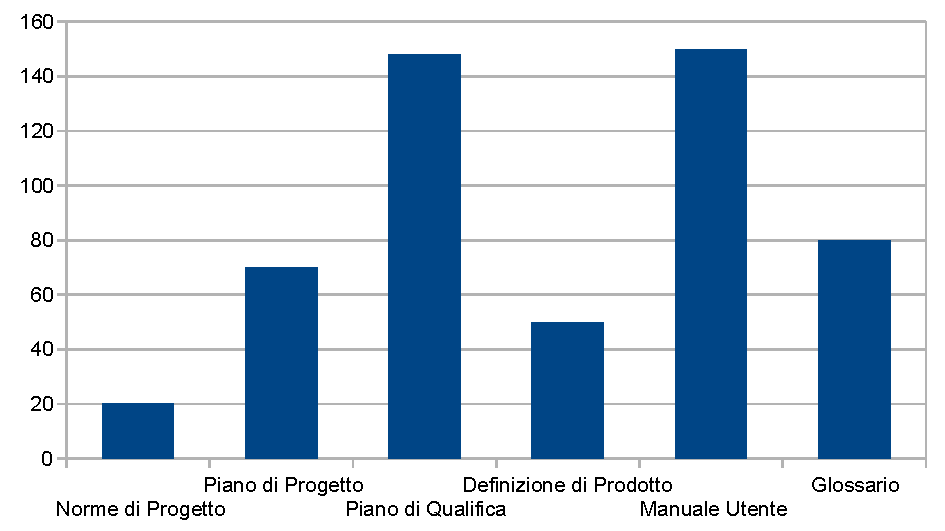
\includegraphics[width=12cm]{PianoDiQualifica/Pics/ProduttivitaDocumentazioneFasePD.pdf}
					\caption{Produttività del processo di documentazione durante la Fase PD}
				\end{figure}
				La produttività media del processo di documentazione è ulteriormente in diminuzione in quanto nuove sezioni ed eventuali ampliamenti introdotti nei documenti in questa fase sono ridotti al minimo. Ciò contrasta coi livelli di Schedule e Budget Variance a causa del fatto che è stata rivista l'organizzazione dei contenuti dei documenti: questo ha causato uno sforzo non banale da parte dei membri del team.\\
				L'esito del risultato è dunque \textbf{non accettabile}. Ci si prefiggeva infatti di aumentare la produttività rispetto alla fase precedente (obiettivo minimo), e idealmente di aumentarla del 10\% (obiettivo ottimale).

		\level{3}{Processo di verifica}
			\level{4}{Miglioramento costante}
				L'obiettivo che il gruppo si era posto inizialmente era quello di far si che il processo fosse in grado di migliorare continuamente (misurando di volta in volta le sue performance e ponendo obiettivi quantitativi). Per calcolare quanto si è vicini a tale obiettivo è stato scelto di fare uso della scala CMM.\\
				Dopo un'approfondita analisi del processo di verifica da parte del gruppo, possiamo affermare che esso ha raggiunto il terzo livello della scala prevista da CMM.\\
				Tale risultato è \textbf{accettabile} rispetto agli obiettivi posti inizialmente (si voleva arrivare come minimo al livello 2, con il risultato ottimale che sarebbe stato il livello 4).
			\level{4}{Rispetto della pianificazione}
				L'obiettivo che il gruppo si era posto inizialmente era quello di non avere attività e task di processo in ritardo rispetto a quanto è stato pianificato all'interno del \insdoc{Piano di Progetto}. Per calcolare quanto si è vicini a tale obiettivo è stato scelto di fare uso della seguente metrica: Schedule Variance.\\
				Riportiamo di seguito i valori ottenuti calcolando la Schedule Variance sul processo di verifica:
				\begin{table}[H]
					\centering
					\begin{tabu}{| l | c | c |}
						\hline
						Processo 			   & Schedule Variance   \\ \hline \hline
						Processo di verifica   & 3\%                 \\ \hline
					\end{tabu}
					\caption{Esiti del calcolo della Schedule Variance sul processo di verifica durante la Fase PD}
				\end{table}
				Possiamo concludere che le attività pianificate nel \insdoc{Piano di Progettov7.00}, relative alla verifica, sono state svolte con un ritardo minimo rispetto ai tempi previsti.\\
				L'esito del risultato è dunque \textbf{accettabile}. Ci si prefiggeva infatti di avere una Schedule variance che valesse al massimo 5\% (obiettivo minimo), e idealmente al massimo 0\% (obiettivo ottimale).	

			\level{4}{Rispetto del budget}
				L'obiettivo che il gruppo si era posto inizialmente era quello di avere un processo che rientrasse nel budget assegnato dal \insdoc{Piano di Progetto}. Per calcolare quanto si è vicini a tale obiettivo è stato scelto di fare uso della seguente metrica: Budget Variance.\\
				Riportiamo di seguito i valori ottenuti calcolando la Budget Variance sul processo di verifica:
				\begin{table}[H]
					\centering
					\begin{tabu}{| l | c | c |}
						\hline
						Processo 			   & Budget Variance     \\ \hline \hline
						Processo di verifica   & 6\%                 \\ \hline
					\end{tabu}
					\caption{Esiti del calcolo della Budget Variance sul processo di verifica durante la Fase PD}
				\end{table}
				Possiamo concludere il processo di verifica non ha rispettato il budget assegnato (seppur di poco). Non c'è stato dunque alcun risparmio, ma solo una piccola perdita. Questo è stato causato dalla necessità di correggere gli errori rilevati durante la Revisione di Qualifica.\\
				L'esito del risultato è dunque \textbf{accettabile}. Ci si prefiggeva infatti di avere una Budget Variance che valesse al massimo 10\% (obiettivo minimo), e idealmente al massimo 0\% (obiettivo ottimale).

			\level{4}{Efficacia ed efficienza}
				L'obiettivo che il gruppo si era posto inizialmente era quello di far si che il processo fosse sia efficiente che efficace. Per calcolare quanto si è vicini a tale obiettivo è stato scelto di fare uso delle seguenti metriche:
				\begin{itemize}
					\item produttività;
					\item efficacia di una revisione.
				\end{itemize}
				Utilizzando la formula descritta all'interno del presente documento (sezione \nameref{subsec:produttivita}) è stata calcolata la produttività del processo di verifica. Questo indice è stato calcolato durante tutti i momenti di verifica previsti dal \insdoc{Piano di Progetto v7.00}.Riassumendo i risultati:
				\begin{table}[H]
			    	\centering
					\begin{tabu}{| c | c |}
						\hline
						Data verifica   & Produttività   \\ \hline \hline
						01/06-02/06     & 3              \\ \hline
						03/06-05/06     & 10             \\ \hline
						06/06-11/06     & 16             \\ \hline
						11/06-16/06     & 5              \\ \hline
					\end{tabu}
					\caption{Produttività del processo di verifica durante la fase PD}
				\end{table}
				Di seguito vengono riportati in un grafico i valori della produttività del processo di verifica rilevati nei vari periodi della \insphase{Fase PD}. Il grafico fa riferimento alla tabella precedente.
				\begin{figure}[H]
					\centering
					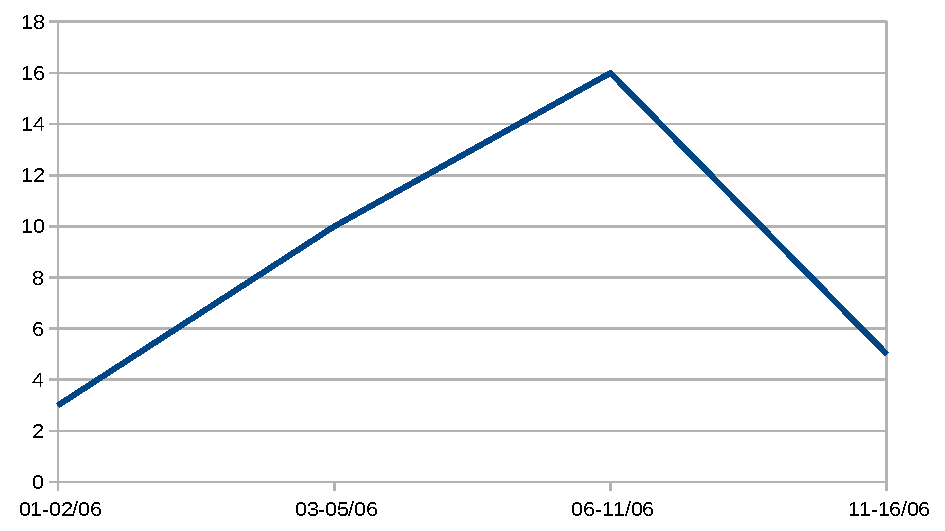
\includegraphics[width=12cm]{PianoDiQualifica/Pics/ProduttivitaVerificaFasePD.pdf}
					\caption{Produttività del processo di verifica durante la Fase PD}
				\end{figure}
				La produttività ha avuto un picco finale dovuto alla necessità di rivedere i documenti presentati alla Revisione di Qualifica, in seguito alle valutazioni ricevute in quel periodo, e alla necessità di verificare il codice prodotto. Si può notare che il livello di produttività è, in media, di poco superiore rispetto alle fasi precedenti.\\
				L'esito del risultato è dunque \textbf{accettabile}. Ci si prefiggeva infatti di aumentare la produttività rispetto alla fase precedente (obiettivo minimo), e idealmente di aumentarla del 10\% (obiettivo ottimale).\\
				Utilizzando la formula descritta all'interno del presente documento (sezione \nameref{subsec:effRevisione}) è stata calcolata l'efficacia delle varie revisioni che sono state fatte durante la \insphase{Fase PD}. Di seguito vengono riportati i valori calcolati:
				\begin{table}[H]
					\centering
					\begin{tabu}{| c | c |}
						\hline
						Data verifica   & Efficacia della revisione   \\ \hline \hline
						01/06-02/06     & 6                           \\ \hline
						03/06-05/06     & 10                          \\ \hline
						06/06-11/06     & 18                          \\ \hline
						12/06-16/06     & 8                           \\ \hline
					\end{tabu}
					\caption{Efficacia delle revisioni durante la fase PD}
				\end{table}
				Di seguito viene riportata una rappresentazione grafica dei valori calcolati precedentemente.
				\begin{figure}[H]
					\centering
					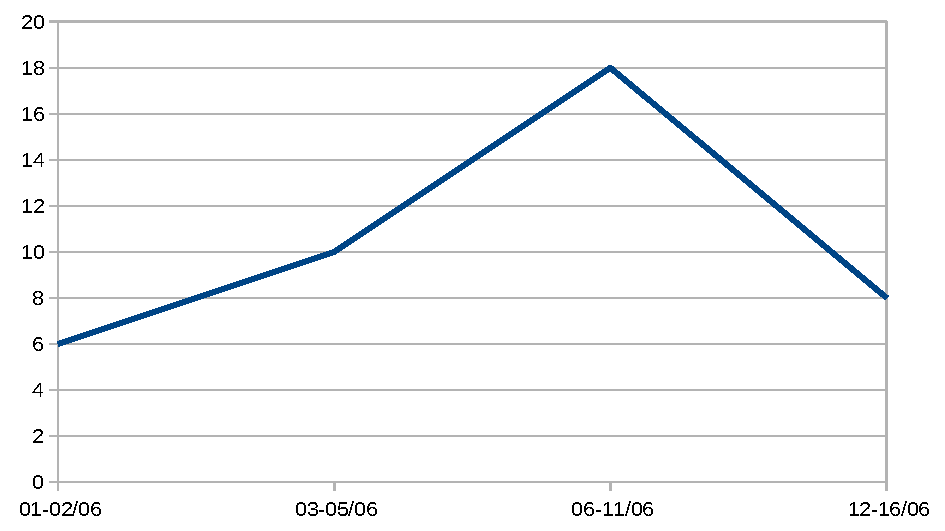
\includegraphics[width=12cm]{PianoDiQualifica/Pics/EfficaciaRevisioniFasePD.pdf}
					\caption{Efficacia delle revisioni durante la Fase PD}
				\end{figure}
				I livelli di efficacia di revisione, nel complesso, rispecchiano l'andamento della produttività. Essi sono in media di poco superiori a quelli calcolati in precedenza. Si noti il picco nel momento in cui sono state apportate modifiche in seguito alle valutazioni ricevute dopo la Revisione di Qualifica.\\
				L'esito del risultato è dunque \textbf{ottimale}. Ci si prefiggeva infatti di aumentare la l'efficacia di una revisione rispetto alla fase precedente (obiettivo minimo), e idealmente di aumentarla del 5\% (obiettivo ottimale).

		\level{3}{Processo di sviluppo}
			\level{4}{Miglioramento costante}
				L'obiettivo che il gruppo si era posto inizialmente era quello di far si che il processo fosse in grado di migliorare continuamente (misurando di volta in volta le sue performance e ponendo obiettivi quantitativi). Per calcolare quanto si è vicini a tale obiettivo è stato scelto di fare uso della scala CMM.\\
				Dopo un'approfondita analisi del processo di sviluppo da parte del gruppo, possiamo affermare che esso ha raggiunto il quarto livello della scala prevista da CMM.\\
				Tale risultato è \textbf{ottimale} rispetto agli obiettivi posti inizialmente (si voleva arrivare come minimo al livello 2, con il risultato ottimale che sarebbe stato il livello 4).
			
			\level{4}{Rispetto della pianificazione}
				L'obiettivo che il gruppo si era posto inizialmente era quello di non avere attività e task di processo in ritardo rispetto a quanto è stato pianificato all'interno del \insdoc{Piano di Progetto}. Per calcolare quanto si è vicini a tale obiettivo è stato scelto di fare uso della seguente metrica: Schedule Variance.\\
				Riportiamo di seguito i valori ottenuti calcolando la Schedule Variance sul processo di sviluppo:
				\begin{table}[H]
					\centering
					\begin{tabu}{| l | c | c |}
						\hline
						Processo 			   & Schedule Variance   \\ \hline \hline
						Processo di sviluppo   & -7\%                \\ \hline
					\end{tabu}
					\caption{Esiti del calcolo della Schedule Variance sul processo di sviluppo durante la Fase PD}
				\end{table}
				Possiamo concludere che le attività pianificate nel \insdoc{Piano di Progettov7.00}, relative allo sviluppo, sono state svolte in minor tempo rispetto a quanto pianificato (la codifica ha impiegato molto meno tempo del previsto, avendo a disposizione una buona progettazione di dettaglio).\\
				L'esito del risultato è dunque \textbf{ottimale}. Ci si prefiggeva infatti di avere una Schedule variance che valesse al massimo 5\% (obiettivo minimo), e idealmente al massimo 0\% (obiettivo ottimale).
						
			\level{4}{Rispetto del budget}
				L'obiettivo che il gruppo si era posto inizialmente era quello di avere un processo che rientrasse nel budget assegnato dal \insdoc{Piano di Progetto}. Per calcolare quanto si è vicini a tale obiettivo è stato scelto di fare uso della seguente metrica: Budget Variance.\\
				Riportiamo di seguito i valori ottenuti calcolando la Budget Variance sul processo di sviluppo:
				\begin{table}[H]
					\centering
					\begin{tabu}{| l | c | c |}
						\hline
						Processo 			   & Budget Variance     \\ \hline \hline
						Processo di sviluppo   & -4\%                 \\ \hline
					\end{tabu}
					\caption{Esiti del calcolo della Budget Variance sul processo di sviluppo durante la Fase PD}
				\end{table}
				Possiamo concludere il processo di sviluppo ha fatto si che si risparmiasse una piccola somma rispetto al budget assegnato. La codifica infatti ha impiegato molto meno tempo del previsto (e di conseguenza anche i costi si sono abbassati), avendo a disposizione una buona progettazione di dettaglio\\
				L'esito del risultato è dunque \textbf{ottimale}. Ci si prefiggeva infatti di avere una Budget Variance che valesse al massimo 10\% (obiettivo minimo), e idealmente al massimo 0\% (obiettivo ottimale).
							
			\level{4}{Efficacia ed efficienza}
				L'obiettivo che il gruppo si era posto inizialmente era quello di far si che il processo fosse sia efficiente che efficace. Per calcolare quanto si è vicini a tale obiettivo è stato scelto di fare uso della seguente metrica: produttività.\\
				Utilizzando la formula descritta all'interno del presente documento (sezione \nameref{subsec:produttivita}) è stata calcolata la produttività del processo di sviluppo. Questo indice è stato calcolato per ognuna delle attività previste da tale processo in questa fase. Il calcolo è stato fatto di volta in volta solo sui nuovi prodotti, senza tenere conto di quelli vecchi. Riassumendo i risultati:
				\begin{table}[H]
			    	\centering
					\begin{tabu}{| l | c | c |}
						\hline
						Attività di processo   & Produttività   \\ \hline \hline
						Codifica               & 46             \\ \hline
						Progettazione          & 95             \\ \hline
					\end{tabu}
				\caption{Esiti del calcolo della produttività del processo di sviluppo durante la Fase PD}
				\end{table}
				La produttività del processo di sviluppo è aumentata mediamente del 17\% rispetto alla fase precedente. Questo è dovuto in parte al leggero miglioramento nella produttività della codifica, in parte dal fatto che la progettazione è stata molto efficace ed efficiente (il compito è stato semplificato da alcuni incontri con il proponente che ci ha fatto aprire gli occhi su alcuni aspetti critici).\\
				L'esito del risultato è dunque \textbf{ottimale}. Ci si prefiggeva infatti di aumentare la produttività rispetto alla fase precedente (obiettivo minimo), e idealmente di aumentarla del 10\% (obiettivo ottimale).
			
		\level{3}{Processo di validazione}
			\level{4}{Miglioramento costante}
				L'obiettivo che il gruppo si era posto inizialmente era quello di far si che il processo fosse in grado di migliorare continuamente (misurando di volta in volta le sue performance e ponendo obiettivi quantitativi). Per calcolare quanto si è vicini a tale obiettivo è stato scelto di fare uso della scala CMM.\\
				Dopo un'approfondita analisi del processo di validazione da parte del gruppo, possiamo affermare che esso ha raggiunto il secondo livello della scala prevista da CMM.\\
				Tale risultato è \textbf{accettabile} rispetto agli obiettivi posti inizialmente (si voleva arrivare come minimo al livello 2, con il risultato ottimale che sarebbe stato il livello 4).\\
				Questo processo è stato attuato solo per un breve periodo, ed è per questo motivo che il suo livello CMM è così basso rispetto agli altri processi: il gruppo è consapevole di non aver ancora acquisito sufficiente padronanza del processo stesso.
			
			\level{4}{Rispetto della pianificazione}
				L'obiettivo che il gruppo si era posto inizialmente era quello di non avere attività e task di processo in ritardo rispetto a quanto è stato pianificato all'interno del \insdoc{Piano di Progetto}. Per calcolare quanto si è vicini a tale obiettivo è stato scelto di fare uso della seguente metrica: Schedule Variance.\\
				Riportiamo di seguito i valori ottenuti calcolando la Schedule Variance sul processo di validazione:
				\begin{table}[H]
					\centering
					\begin{tabu}{| l | c | c |}
						\hline
						Processo 			      & Schedule Variance   \\ \hline \hline
						Processo di validazione   & 0\%                 \\ \hline
					\end{tabu}
					\caption{Esiti del calcolo della Schedule Variance sul processo di validazione durante la Fase PD}
				\end{table}
				Possiamo concludere che le attività pianificate nel \insdoc{Piano di Progettov7.00}, relative alla validazione, sono state svolte in linea con i tempi previsti.\\
				L'esito del risultato è dunque \textbf{ottimale}. Ci si prefiggeva infatti di avere una Schedule variance che valesse al massimo 5\% (obiettivo minimo), e idealmente al massimo 0\% (obiettivo ottimale).
						
			\level{4}{Rispetto del budget}
				L'obiettivo che il gruppo si era posto inizialmente era quello di avere un processo che rientrasse nel budget assegnato dal \insdoc{Piano di Progetto}. Per calcolare quanto si è vicini a tale obiettivo è stato scelto di fare uso della seguente metrica: Budget Variance.\\
				Riportiamo di seguito i valori ottenuti calcolando la Budget Variance sul processo di validazione:
				\begin{table}[H]
					\centering
					\begin{tabu}{| l | c | c |}
						\hline
						Processo 			      & Budget Variance     \\ \hline \hline
						Processo di validazione   & 0\%                 \\ \hline
					\end{tabu}
					\caption{Esiti del calcolo della Budget Variance sul processo di validazione durante la Fase PD}
				\end{table}
				Possiamo concludere il processo di verifica ha rispettato perfettamente il budget assegnato. Non c'è stato dunque alcun risparmio, ma nemmeno perdite. Questo è sintomo di una buona pianificazione.\\
				L'esito del risultato è dunque \textbf{ottimale}. Ci si prefiggeva infatti di avere una Budget Variance che valesse al massimo 10\% (obiettivo minimo), e idealmente al massimo 0\% (obiettivo ottimale).
							
			\level{4}{Efficacia ed efficienza}
				L'obiettivo che il gruppo si era posto inizialmente era quello di far si che il processo fosse sia efficiente che efficace. Per calcolare quanto si è vicini a tale obiettivo è stato scelto di fare uso della seguente metrica: produttività.\\
				Utilizzando la formula descritta all'interno del presente documento (sezione \nameref{subsec:produttivita}) è stata calcolata la produttività del processo di validazione. Questo indice è stato calcolato una sola volta, in linea con quanto previsto dal \insdoc{Piano di Progetto}. Riassumendo i risultati:
				\begin{table}[H]
			    	\centering
					\begin{tabu}{| l | c | c |}
						\hline
							Processi 				  & Produttività   \\ \hline \hline
							Processo di validazione   & 1              \\ \hline
					\end{tabu}
					\caption{Esiti del calcolo della produttività della codifica durante la Fase PD}
				\end{table}
				La produttività del processo di validazione non può essere confrontata con alcun valore, in quanto è la prima volta che essa viene calcolata. Non è dunque possibile affermare se i risultati siano accettabili oppure no seguendo le metriche che sono state adottate.\\
				Tuttavia possiamo comunque affermare che questo risultato è \textbf{ottimale}, in quanto utilizzando la formula che è stata precedentemente introdotta non si possono ottenere risultati maggiori di questo.
		\level{3}{Panoramica degli esiti ottenuti}
			Riportiamo in seguito una tabella che riassume gli esiti della verifica fatta sui vari processi. Tale riassunto è di aiuto al \insrole{Responsabile di Progetto} nel momento in cui egli deve prendere decisioni e imporre obiettivi quantitativi di miglioramento.
			\begin{table}[H]
				\centering
				\begin{tabu}{| l | l | l | c |}
					\hline
					Processo & Obiettivo & Metrica & Esito \\ \hline \hline
					\multirow{4}{*}{Documentazione} 
					& Miglioramento costante        & CMM                       & Accettabile    \\ \cline{2-4}
					& Rispettare la pianificazione  & Schedule Variance         & Ottimale       \\ \cline{2-4}
					& Rispettare il budget          & Budget Variance           & Ottimale       \\ \cline{2-4}
					& Efficacia ed efficienza       & Produttività              & Non accetabile \\ \hline
					\multirow{5}{*}{Verifica}
					& Miglioramento costante        & CMM                       & Accettabile    \\ \cline{2-4}
					& Rispettare la pianificazione  & Schedule Variance         & Accettabile    \\ \cline{2-4}
					& Rispettare il budget          & Budget Variance           & Accettabile    \\ \cline{2-4}
					& \multirow{2}{*}{Efficacia ed efficienza}
													& Produttività              & Accettabile    \\ \cline{3-4}
												  & & Efficacia revisione       & Ottimale       \\ \hline
					\multirow{4}{*}{Sviluppo}
					& Miglioramento costante        & CMM                       & Ottimale       \\ \cline{2-4}
					& Rispettare la pianificazione  & Schedule Variance         & Ottimale       \\ \cline{2-4}
					& Rispettare il budget          & Budget Variance           & Ottimale       \\ \cline{2-4}
					& Efficacia ed efficienza       & Produttività              & Ottimale       \\ \hline
					\multirow{4}{*}{Validazione}
					& Miglioramento costante        & CMM                       & Accettabile    \\ \cline{2-4}
					& Rispettare la pianificazione  & Schedule Variance         & Ottimale       \\ \cline{2-4}
					& Rispettare il budget          & Budget Variance           & Ottimale       \\ \cline{2-4}
					& Efficacia ed efficienza       & Produttività              & Ottimale       \\ \hline
				\end{tabu}
				\caption{Panoramica degli esiti ottenuti nella verifica dei processi durante la fase PD}
			\end{table}